
\documentclass{article}
\usepackage[utf8]{inputenc}
\usepackage[spanish.mexico]{babel}

\title{Dispositivos}
\author{Pablo Vivar Colina}
\date{Septiembre 2017}

\usepackage{natbib}
\usepackage{graphicx}

%Circuitos
\usepackage{tikz}

\usepackage[american voltages, american currents,siunitx]{circuitikz}

%Plotting

\usepackage{pgfplots}
\pgfplotsset{width=10cm,compat=1.9} 
 \usepgfplotslibrary{external}
\tikzexternalize 


%\maketitle

%\usepackage[top=2cm,bottom=2cm,left=1cm,right=1cm]{geometry}


\begin{titlepage}
     \begin{center}
	
\includegraphics[width=0.09\textwidth]{UNAM}\Large Universidad Nacional Autónoma de México
        	
\includegraphics[width=0.09\textwidth]{FI}\\[1cm]
        \Large Facultad de Ingeniería\\[1cm]
       % \Large División de Ciencias Básicas\\[1cm]
         \Large Laboratorio de Fundamentos de Control(6655)\\[1cm]
         %la clave antes era:4314
         \footnotesize Profesor: Salcedo Ubilla María Leonor Ing.\\[1cm]
        \footnotesize Semestre 2019-1\\[1cm]
        
       

        \Large Práctica No. 1\\[1cm]
        
           

\Large Introdcción MATLAB
        
         %Texto a la derecha
          \begin{flushright}
\footnotesize  Grupo 2\\[0.5cm]
\footnotesize Brigada: 4\\[0.5cm]
\footnotesize Rodrigo Adrián Martínez López\\[0.5cm]
\footnotesize Vivar Colina Pablo\\[0.5cm]
 \end{flushright}
    %Texto a la izquierda
          \begin{flushleft}
        \footnotesize Ciudad Universitaria Agosto de 2018.\\
          \end{flushleft}
         
          
        %\vfill
        %\today
   \end{center}
\end{titlepage}
 %agregar portada

\begin{document}

\tableofcontents  % Write out the Table of Contents

\listoffigures  % Write out the List of Figures


\section{Marco Teórico}

\subsection{Oscilación Senoidal}

Una señal senoidal o sinusoidal, $a(t)$, tensión, $v(t)$, o corriente, $i(t)$, se puede expresar matemáticamente según sus parámetros característicos (figura \ref{fig:ondaSenoidal}), como una función del tiempo por medio de la siguiente ecuación:\citep{CA}

\begin{equation}
    a(t)=A_0 \cdot \sin(\omega t + \beta)
\end{equation}
\begin{itemize}
    \item $A_0$ es la ''amplitud'' en [V] o [A] (también llamado ''valor máximo o de pico'')
    
    \item $\omega$  pulsación en radianes/segundo
    
    \item $t$ el tiempo en [s]
    
    \item $\beta$ el ángulo de fase inicial en radianes.
\end{itemize}


Dado que la velocidad angular es más interesante para matemáticos que para ingenieros, la fórmula anterior se suele expresar como:\citep{CA}\\

\begin{equation}
    a(t)=A_0 \cdot \sin(2 \pi f t + \beta)
\end{equation}


donde ''f'' es la frecuencia (Hz) y equivale a la inversa del período $f=\frac{1}{T}$. Los valores más empleados en la distribución son 50 Hz y 60 Hz.\citep{CA}\\

\begin{figure}[ht!]
    \centering
    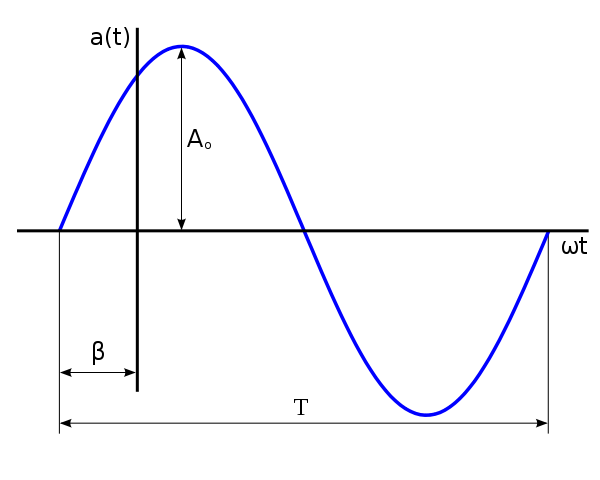
\includegraphics[scale=0.5]{Imagenes/600px-OndaSenoidal.png}
    \caption{Parámetros característicos de una oscilación sinusoidal.}
    \label{fig:ondaSenoidal}
\end{figure}


\section{Desarrollo}

\subsection{Señal Senoidal}

En el primer experimento que se muestra en la figura \ref{Seno7RMS} se utilizó una señal con las siguientes características:\\

\begin{itemize}
    \item Vp=4.9497 [V]
    \item $V_{RMS}$=7 [V]
    \item frecuencia= 1[kHz]
    \item periodo 1 [ms]
\end{itemize}

\begin{figure}[h!]
    \centering

\begin{tikzpicture}
\begin{axis}[
    axis lines = left,
    xlabel = {t[ms]},
    ylabel = {V[V]},
]

\addplot
[thick=0.1cm,
    domain=0:2, 
    samples=100, 
    color=red,
]
{4.9497*sin(deg((2*3.1459*x))};
\addlegendentry{$4.9497 V_{p}$}

\end{axis}
\end{tikzpicture}
\caption{Señal senoidal con $7 V_{RMS}
$ y 1 [kHz]}
\label{Seno7RMS}
\end{figure}




%Segunda seno
También se generó otra señal senoidal con careacterísticas diferentes, se muestra en la figura \ref{Seno3RMS} ´estos cambios de parámetros se reflejan a continuación:\\

\begin{itemize}
    \item Vp=4.24 [V]
    \item $V_{RMS}$=3 [V]
    \item frecuencia= 20[kHz]
    \item periodo 1 [ms]
\end{itemize}


\begin{figure}[h!]
    \centering
    
   
\begin{tikzpicture}
\begin{axis}[
    axis lines = left,
    xlabel = {t[ms]},
    ylabel = {V[V]},
]

\addplot
[thick=0.1cm,
    domain=0:2, 
    samples=100, 
    color=blue,
]
{4.24*sin(deg((40*3.1459*x))};
%\addlegendentry{$4.9497 V_{p}$}

\end{axis}
\end{tikzpicture}
\caption{Señal senoidal con $3 V_{RMS}$ y 20 [kHz]}
\label{Seno3RMS}
\end{figure}


\subsection{Señal Cuadrada}

Para éste experimento se tomaron las señales generadas en el experimento anterior y se unieron.

%%%##### EXPERIMENTO#######


\begin{figure}[h!]
    \centering
    
   
\begin{tikzpicture}
\begin{axis}[
    axis lines = left,
    xlabel = {t[ms]},
    ylabel = {V[V]},
]

\addplot
[thick=0.1cm,
    domain=0:2, 
    samples=100, 
    color=green,
]
{4.9497*sin(deg((2*3.1459*x))+4.24*sin(deg((40*3.1459*x))};

\end{axis}
\end{tikzpicture}
\caption{Espectro ideal de la suma de las señales de las figuras \ref{Seno7RMS} y \ref{Seno3RMS}  }
\end{figure}


\begin{figure}[h!]
    \centering
    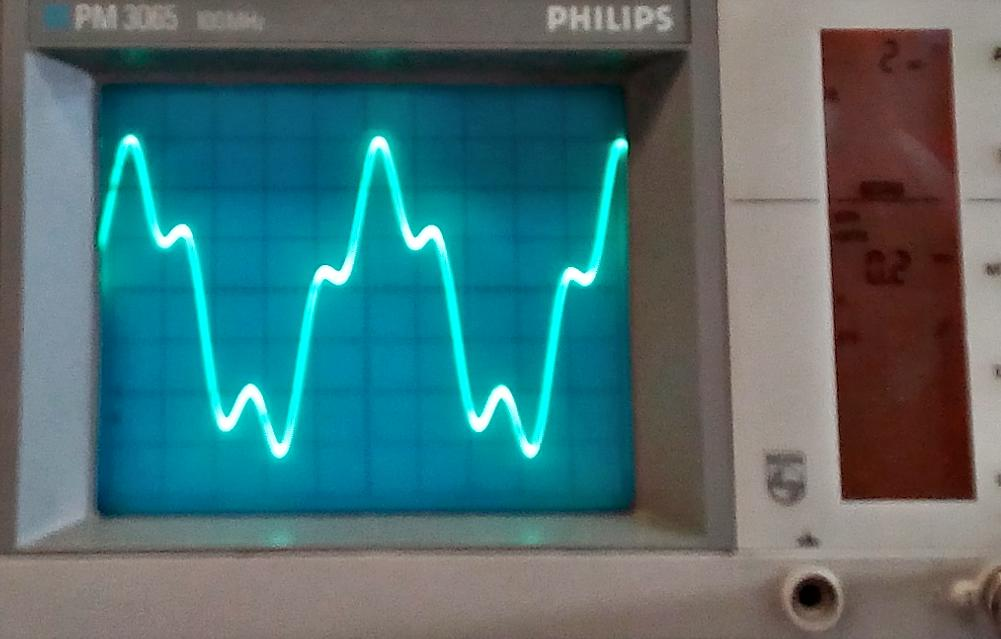
\includegraphics[scale=0.25]{Imagenes/FrecSin.jpg}
    \caption{Espectro en osciloscopio de la suma de las señales de las figuras \ref{Seno7RMS} y \ref{Seno3RMS} }
    \label{fig:SenalCOmb}
\end{figure}

\begin{figure}[h!]
    \centering
    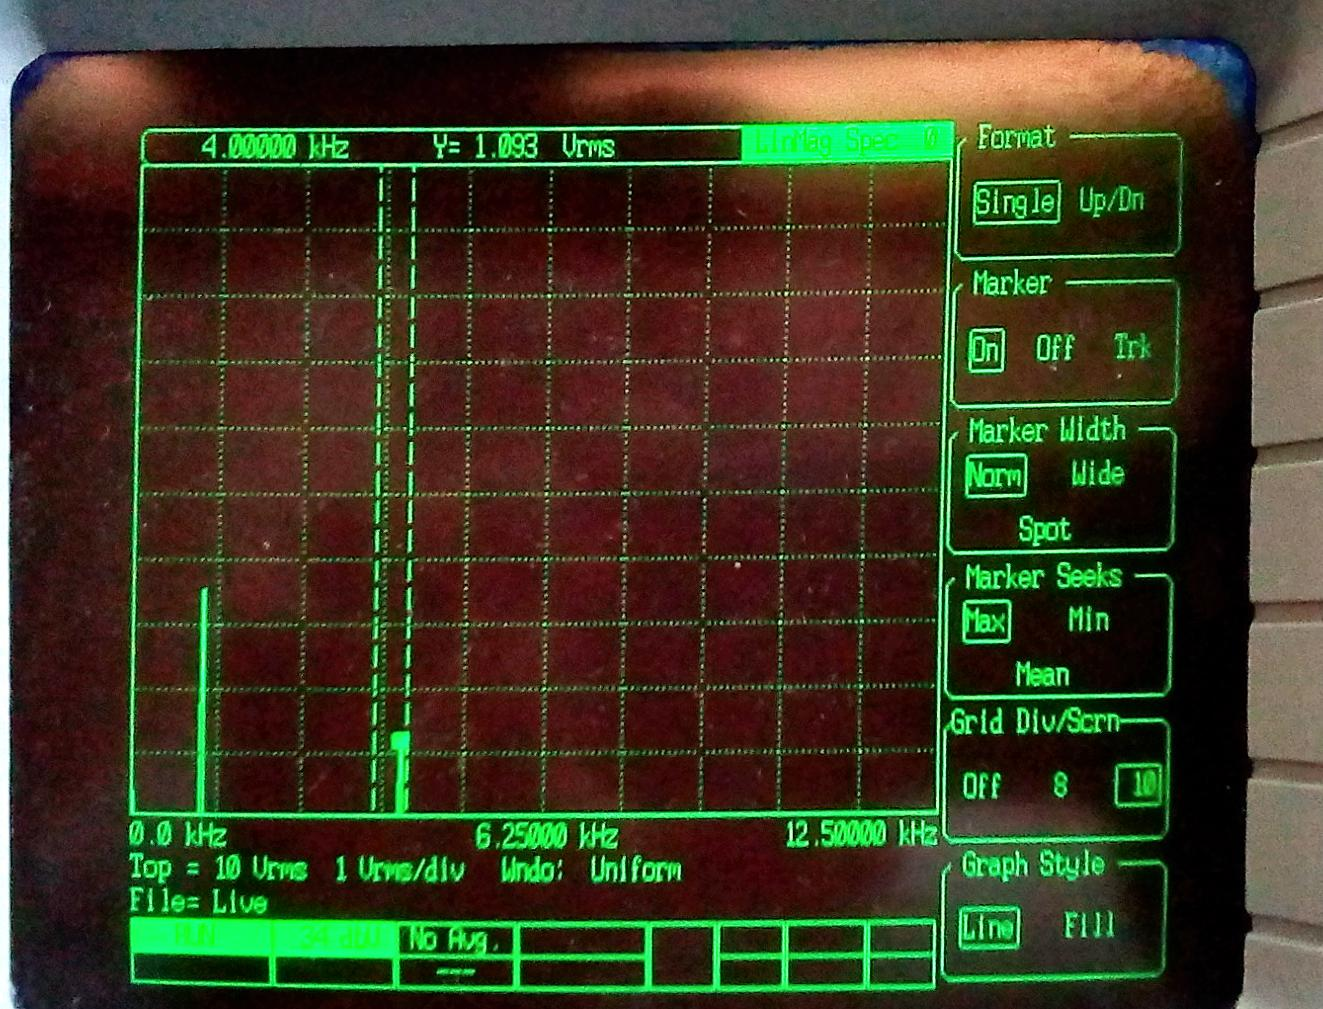
\includegraphics[scale=0.15]{Imagenes/Frec1.jpg}
    \caption{Espectro en frecuencias de la figura \ref{fig:SenalCOmb}}
    \label{fig:my_label}
\end{figure}

\begin{figure}[h!]
    \centering
    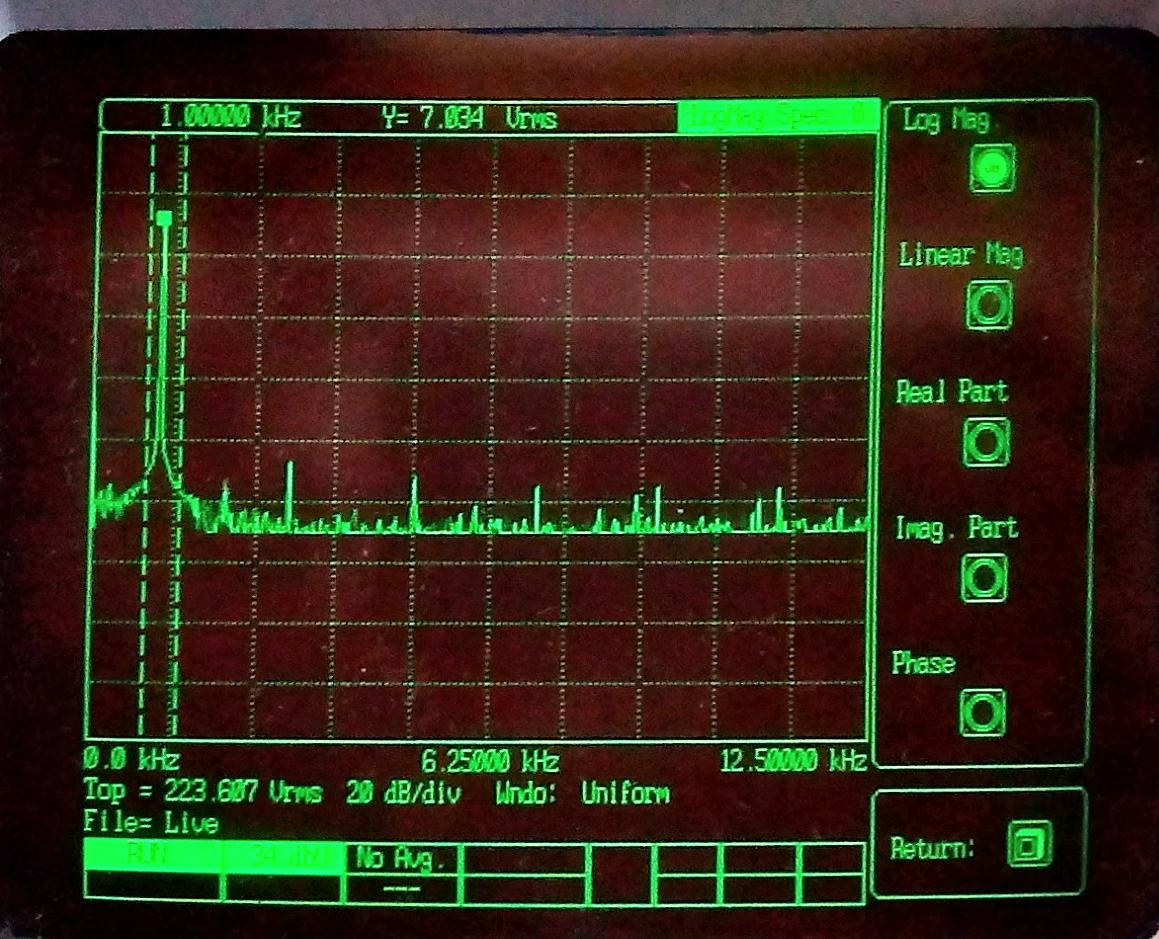
\includegraphics[scale=0.15]{Imagenes/FrecSenPur.jpg}
    \caption{Espectro en frecuencias de la señal obtenida el la figura \ref{Seno7RMS}}
    \label{fig:frecuenciasSeno}
\end{figure}



\section{Conclusiones}

La práctica de análisis espectral de señales fué satisfactoria porque logramos ver la señal senoidal con distintos parámetros y ver su comportamiento en el generador de espectro, también cómo la señal cuadrada está representada por varias funciones senoidales.

Logramos ver también la combinación de dos señales senoidales y ver su espectro en el osciloscopio y en el analizador de espectros.

\section{Comentarios}

Es necesario un buen manejo del equipo, en particular del analizador de espectros ya que es un equipo que en los laboratorios anteriores no se ha utilizado, y que es importante para comprender la suma de señales con diferentes frecuencias.

%.\\[100cm]
\bibliographystyle{plain}
\bibliography{Referencias.bib}

\end{document}
